%% template.tex
%% from
%% bare_conf.tex
%% V1.4b
%% 2015/08/26
%% by Michael Shell
%% See:
%% http://www.michaelshell.org/
%% for current contact information.
%%
%% This is a skeleton file demonstrating the use of IEEEtran.cls
%% (requires IEEEtran.cls version 1.8b or later) with an IEEE
%% conference paper.
%%
%% Support sites:
%% http://www.michaelshell.org/tex/ieeetran/
%% http://www.ctan.org/pkg/ieeetran
%% and
%% http://www.ieee.org/

%%*************************************************************************
%% Legal Notice:
%% This code is offered as-is without any warranty either expressed or
%% implied; without even the implied warranty of MERCHANTABILITY or
%% FITNESS FOR A PARTICULAR PURPOSE!
%% User assumes all risk.
%% In no event shall the IEEE or any contributor to this code be liable for
%% any damages or losses, including, but not limited to, incidental,
%% consequential, or any other damages, resulting from the use or misuse
%% of any information contained here.
%%
%% All comments are the opinions of their respective authors and are not
%% necessarily endorsed by the IEEE.
%%
%% This work is distributed under the LaTeX Project Public License (LPPL)
%% ( http://www.latex-project.org/ ) version 1.3, and may be freely used,
%% distributed and modified. A copy of the LPPL, version 1.3, is included
%% in the base LaTeX documentation of all distributions of LaTeX released
%% 2003/12/01 or later.
%% Retain all contribution notices and credits.
%% ** Modified files should be clearly indicated as such, including  **
%% ** renaming them and changing author support contact information. **
%%*************************************************************************


% *** Authors should verify (and, if needed, correct) their LaTeX system  ***
% *** with the testflow diagnostic prior to trusting their LaTeX platform ***
% *** with production work. The IEEE's font choices and paper sizes can   ***
% *** trigger bugs that do not appear when using other class files.       ***                          ***
% The testflow support page is at:
% http://www.michaelshell.org/tex/testflow/

\documentclass[conference,final,]{IEEEtran}
% Some Computer Society conferences also require the compsoc mode option,
% but others use the standard conference format.
%
% If IEEEtran.cls has not been installed into the LaTeX system files,
% manually specify the path to it like:
% \documentclass[conference]{../sty/IEEEtran}





% Some very useful LaTeX packages include:
% (uncomment the ones you want to load)


% *** MISC UTILITY PACKAGES ***
%
%\usepackage{ifpdf}
% Heiko Oberdiek's ifpdf.sty is very useful if you need conditional
% compilation based on whether the output is pdf or dvi.
% usage:
% \ifpdf
%   % pdf code
% \else
%   % dvi code
% \fi
% The latest version of ifpdf.sty can be obtained from:
% http://www.ctan.org/pkg/ifpdf
% Also, note that IEEEtran.cls V1.7 and later provides a builtin
% \ifCLASSINFOpdf conditional that works the same way.
% When switching from latex to pdflatex and vice-versa, the compiler may
% have to be run twice to clear warning/error messages.






% *** CITATION PACKAGES ***
%
%\usepackage{cite}
% cite.sty was written by Donald Arseneau
% V1.6 and later of IEEEtran pre-defines the format of the cite.sty package
% \cite{} output to follow that of the IEEE. Loading the cite package will
% result in citation numbers being automatically sorted and properly
% "compressed/ranged". e.g., [1], [9], [2], [7], [5], [6] without using
% cite.sty will become [1], [2], [5]--[7], [9] using cite.sty. cite.sty's
% \cite will automatically add leading space, if needed. Use cite.sty's
% noadjust option (cite.sty V3.8 and later) if you want to turn this off
% such as if a citation ever needs to be enclosed in parenthesis.
% cite.sty is already installed on most LaTeX systems. Be sure and use
% version 5.0 (2009-03-20) and later if using hyperref.sty.
% The latest version can be obtained at:
% http://www.ctan.org/pkg/cite
% The documentation is contained in the cite.sty file itself.






% *** GRAPHICS RELATED PACKAGES ***
%
\ifCLASSINFOpdf
  % \usepackage[pdftex]{graphicx}
  % declare the path(s) where your graphic files are
  % \graphicspath{{../pdf/}{../jpeg/}}
  % and their extensions so you won't have to specify these with
  % every instance of \includegraphics
  % \DeclareGraphicsExtensions{.pdf,.jpeg,.png}
\else
  % or other class option (dvipsone, dvipdf, if not using dvips). graphicx
  % will default to the driver specified in the system graphics.cfg if no
  % driver is specified.
  % \usepackage[dvips]{graphicx}
  % declare the path(s) where your graphic files are
  % \graphicspath{{../eps/}}
  % and their extensions so you won't have to specify these with
  % every instance of \includegraphics
  % \DeclareGraphicsExtensions{.eps}
\fi
% graphicx was written by David Carlisle and Sebastian Rahtz. It is
% required if you want graphics, photos, etc. graphicx.sty is already
% installed on most LaTeX systems. The latest version and documentation
% can be obtained at:
% http://www.ctan.org/pkg/graphicx
% Another good source of documentation is "Using Imported Graphics in
% LaTeX2e" by Keith Reckdahl which can be found at:
% http://www.ctan.org/pkg/epslatex
%
% latex, and pdflatex in dvi mode, support graphics in encapsulated
% postscript (.eps) format. pdflatex in pdf mode supports graphics
% in .pdf, .jpeg, .png and .mps (metapost) formats. Users should ensure
% that all non-photo figures use a vector format (.eps, .pdf, .mps) and
% not a bitmapped formats (.jpeg, .png). The IEEE frowns on bitmapped formats
% which can result in "jaggedy"/blurry rendering of lines and letters as
% well as large increases in file sizes.
%
% You can find documentation about the pdfTeX application at:
% http://www.tug.org/applications/pdftex

\usepackage{graphicx}

% *** MATH PACKAGES ***
%
\usepackage{amsmath}
\interdisplaylinepenalty=2500
%\usepackage{amsmath}
% A popular package from the American Mathematical Society that provides
% many useful and powerful commands for dealing with mathematics.
%
% Note that the amsmath package sets \interdisplaylinepenalty to 10000
% thus preventing page breaks from occurring within multiline equations. Use:
%\interdisplaylinepenalty=2500
% after loading amsmath to restore such page breaks as IEEEtran.cls normally
% does. amsmath.sty is already installed on most LaTeX systems. The latest
% version and documentation can be obtained at:
% http://www.ctan.org/pkg/amsmath





% *** SPECIALIZED LIST PACKAGES ***
%
%\usepackage{algorithmic}
% algorithmic.sty was written by Peter Williams and Rogerio Brito.
% This package provides an algorithmic environment fo describing algorithms.
% You can use the algorithmic environment in-text or within a figure
% environment to provide for a floating algorithm. Do NOT use the algorithm
% floating environment provided by algorithm.sty (by the same authors) or
% algorithm2e.sty (by Christophe Fiorio) as the IEEE does not use dedicated
% algorithm float types and packages that provide these will not provide
% correct IEEE style captions. The latest version and documentation of
% algorithmic.sty can be obtained at:
% http://www.ctan.org/pkg/algorithms
% Also of interest may be the (relatively newer and more customizable)
% algorithmicx.sty package by Szasz Janos:
% http://www.ctan.org/pkg/algorithmicx




% *** ALIGNMENT PACKAGES ***
%
%\usepackage{array}
% Frank Mittelbach's and David Carlisle's array.sty patches and improves
% the standard LaTeX2e array and tabular environments to provide better
% appearance and additional user controls. As the default LaTeX2e table
% generation code is lacking to the point of almost being broken with
% respect to the quality of the end results, all users are strongly
% advised to use an enhanced (at the very least that provided by array.sty)
% set of table tools. array.sty is already installed on most systems. The
% latest version and documentation can be obtained at:
% http://www.ctan.org/pkg/array


% IEEEtran contains the IEEEeqnarray family of commands that can be used to
% generate multiline equations as well as matrices, tables, etc., of high
% quality.




% *** SUBFIGURE PACKAGES ***
%\ifCLASSOPTIONcompsoc
%  \usepackage[caption=false,font=normalsize,labelfont=sf,textfont=sf]{subfig}
%\else
%  \usepackage[caption=false,font=footnotesize]{subfig}
%\fi
% subfig.sty, written by Steven Douglas Cochran, is the modern replacement
% for subfigure.sty, the latter of which is no longer maintained and is
% incompatible with some LaTeX packages including fixltx2e. However,
% subfig.sty requires and automatically loads Axel Sommerfeldt's caption.sty
% which will override IEEEtran.cls' handling of captions and this will result
% in non-IEEE style figure/table captions. To prevent this problem, be sure
% and invoke subfig.sty's "caption=false" package option (available since
% subfig.sty version 1.3, 2005/06/28) as this is will preserve IEEEtran.cls
% handling of captions.
% Note that the Computer Society format requires a larger sans serif font
% than the serif footnote size font used in traditional IEEE formatting
% and thus the need to invoke different subfig.sty package options depending
% on whether compsoc mode has been enabled.
%
% The latest version and documentation of subfig.sty can be obtained at:
% http://www.ctan.org/pkg/subfig




% *** FLOAT PACKAGES ***
%

%\usepackage{fixltx2e}
% fixltx2e, the successor to the earlier fix2col.sty, was written by
% Frank Mittelbach and David Carlisle. This package corrects a few problems
% in the LaTeX2e kernel, the most notable of which is that in current
% LaTeX2e releases, the ordering of single and double column floats is not
% guaranteed to be preserved. Thus, an unpatched LaTeX2e can allow a
% single column figure to be placed prior to an earlier double column
% figure.
% Be aware that LaTeX2e kernels dated 2015 and later have fixltx2e.sty's
% corrections already built into the system in which case a warning will
% be issued if an attempt is made to load fixltx2e.sty as it is no longer
% needed.
% The latest version and documentation can be found at:
% http://www.ctan.org/pkg/fixltx2e


%\usepackage{stfloats}
% stfloats.sty was written by Sigitas Tolusis. This package gives LaTeX2e
% the ability to do double column floats at the bottom of the page as well
% as the top. (e.g., "\begin{figure*}[!b]" is not normally possible in
% LaTeX2e). It also provides a command:
%\fnbelowfloat
% to enable the placement of footnotes below bottom floats (the standard
% LaTeX2e kernel puts them above bottom floats). This is an invasive package
% which rewrites many portions of the LaTeX2e float routines. It may not work
% with other packages that modify the LaTeX2e float routines. The latest
% version and documentation can be obtained at:
% http://www.ctan.org/pkg/stfloats
% Do not use the stfloats baselinefloat ability as the IEEE does not allow
% \baselineskip to stretch. Authors submitting work to the IEEE should note
% that the IEEE rarely uses double column equations and that authors should try
% to avoid such use. Do not be tempted to use the cuted.sty or midfloat.sty
% packages (also by Sigitas Tolusis) as the IEEE does not format its papers in
% such ways.
% Do not attempt to use stfloats with fixltx2e as they are incompatible.
% Instead, use Morten Hogholm'a dblfloatfix which combines the features
% of both fixltx2e and stfloats:
%
% \usepackage{dblfloatfix}
% The latest version can be found at:
% http://www.ctan.org/pkg/dblfloatfix




% *** PDF, URL AND HYPERLINK PACKAGES ***
%
%\usepackage{url}
% url.sty was written by Donald Arseneau. It provides better support for
% handling and breaking URLs. url.sty is already installed on most LaTeX
% systems. The latest version and documentation can be obtained at:
% http://www.ctan.org/pkg/url
% Basically, \url{my_url_here}.




% *** Do not adjust lengths that control margins, column widths, etc. ***
% *** Do not use packages that alter fonts (such as pslatex).         ***
% There should be no need to do such things with IEEEtran.cls V1.6 and later.
% (Unless specifically asked to do so by the journal or conference you plan
% to submit to, of course. )



%% BEGIN MY ADDITIONS %%


\usepackage[unicode=true]{hyperref}

\hypersetup{
            pdftitle={Intelligent Automation of SFO Crime Prediction using Multiple AI Methods},
            pdfkeywords={Artificial Intelligence, Machine Learning, Deep
Learning, TabNet, Crime Pattern Theory},
            pdfborder={0 0 0},
            breaklinks=true}
\urlstyle{same}  % don't use monospace font for urls

% Pandoc toggle for numbering sections (defaults to be off)
\setcounter{secnumdepth}{0}


% tightlist command for lists without linebreak
\providecommand{\tightlist}{%
  \setlength{\itemsep}{0pt}\setlength{\parskip}{0pt}}


% Pandoc citation processing
%From Pandoc 3.1.8
% definitions for citeproc citations
\NewDocumentCommand\citeproctext{}{}
\NewDocumentCommand\citeproc{mm}{%
  \begingroup\def\citeproctext{#2}\cite{#1}\endgroup}
\makeatletter
 % allow citations to break across lines
 \let\@cite@ofmt\@firstofone
 % avoid brackets around text for \cite:
 \def\@biblabel#1{}
 \def\@cite#1#2{{#1\if@tempswa , #2\fi}}
\makeatother
\newlength{\cslhangindent}
\setlength{\cslhangindent}{1.5em}
\newlength{\csllabelwidth}
\setlength{\csllabelwidth}{3em}
\newenvironment{CSLReferences}[2] % #1 hanging-indent, #2 entry-spacing
 {\begin{list}{}{%
  \setlength{\itemindent}{0pt}
  \setlength{\leftmargin}{0pt}
  \setlength{\parsep}{0pt}
  % turn on hanging indent if param 1 is 1
  \ifodd #1
   \setlength{\leftmargin}{\cslhangindent}
   \setlength{\itemindent}{-1\cslhangindent}
  \fi
  % set entry spacing
  \setlength{\itemsep}{#2\baselineskip}}}
 {\end{list}}
\usepackage{calc}
\newcommand{\CSLBlock}[1]{#1\hfill\break}
\newcommand{\CSLLeftMargin}[1]{\parbox[t]{\csllabelwidth}{#1}}
\newcommand{\CSLRightInline}[1]{\parbox[t]{\linewidth - \csllabelwidth}{#1}\break}
\newcommand{\CSLIndent}[1]{\hspace{\cslhangindent}#1}


%% END MY ADDITIONS %%


\hyphenation{op-tical net-works semi-conduc-tor}

\begin{document}
%
% paper title
% Titles are generally capitalized except for words such as a, an, and, as,
% at, but, by, for, in, nor, of, on, or, the, to and up, which are usually
% not capitalized unless they are the first or last word of the title.
% Linebreaks \\ can be used within to get better formatting as desired.
% Do not put math or special symbols in the title.
\title{Intelligent Automation of SFO Crime Prediction using Multiple AI
Methods}

% author names and affiliations
% use a multiple column layout for up to three different
% affiliations

\author{

%% ---- classic IEEETrans wide authors' list ----------------
\IEEEauthorblockN{
Praveen Kuruvangi Parameshwara\IEEEauthorrefmark{1},Shilpa Gupta\IEEEauthorrefmark{2}%%
}


%% ----------------------------------------------------------

%% ---- classic IEEETrans one column per institution --------
 %%
%% ----------------------------------------------------------





%% ---- one column per author, classic/default IEEETrans ----

%% ----------------------------------------------------------

}

% conference papers do not typically use \thanks and this command
% is locked out in conference mode. If really needed, such as for
% the acknowledgment of grants, issue a \IEEEoverridecommandlockouts
% after \documentclass

% for over three affiliations, or if they all won't fit within the width
% of the page, use this alternative format:
%
%\author{\IEEEauthorblockN{Michael Shell\IEEEauthorrefmark{1},
%Homer Simpson\IEEEauthorrefmark{2},
%James Kirk\IEEEauthorrefmark{3},
%Montgomery Scott\IEEEauthorrefmark{3} and
%Eldon Tyrell\IEEEauthorrefmark{4}}
%\IEEEauthorblockA{\IEEEauthorrefmark{1}School of Electrical and Computer Engineering\\
%Georgia Institute of Technology,
%Atlanta, Georgia 30332--0250\\ Email: see http://www.michaelshell.org/contact.html}
%\IEEEauthorblockA{\IEEEauthorrefmark{2}Twentieth Century Fox, Springfield, USA\\
%Email: homer@thesimpsons.com}
%\IEEEauthorblockA{\IEEEauthorrefmark{3}Starfleet Academy, San Francisco, California 96678-2391\\
%Telephone: (800) 555--1212, Fax: (888) 555--1212}
%\IEEEauthorblockA{\IEEEauthorrefmark{4}Tyrell Inc., 123 Replicant Street, Los Angeles, California 90210--4321}}




% use for special paper notices
%\IEEEspecialpapernotice{(Invited Paper)}




% make the title area
\maketitle

% As a general rule, do not put math, special symbols or citations
% in the abstract
\begin{abstract}
Crime needs a broad understanding of its patterns and reasons behind
specific types that happen in certain areas only. The crime pattern
theory provides the explanation of distribution of criminal events and
its variations. Crime generators and crime attractor concentrate in the
places that include frequent routine movements of the population to
create hot and cold spots of crime. The offender is more often
comfortable with frequently committed crimes and prefers to commit these
in the places that they are most familiar with. These offenders can be
distinguished based on the type of crimes that fall into specific
incident categories. Identifying these categories help to categorize not
only frequently occurring crime locations but also facilitate the police
department to consider the type of support or action that needs to be
planned. Special analysis of crimes and its categories are essential to
understand the frequency, time and its patterns. This paper showcases
the use of different Artificial Intelligence techniques and compares
their behavior and outcomes which includes different machine learning
and deep learning techniques like random forest, K-nearest neighbor,
Artificial Neural Network, TabNet and Time Series. These are different
flavors of Artificial intelligence and also interactive dashboards and
web applications are supported to visualize the hidden patterns and in
depth details the different features. The flexibility of the paper is
extended to support any type of crime dataset with a minor initial data
streamline process and complete end to end flow is built using only a
python program to reduce the infrastructure cost.
\end{abstract}

% keywords
\begin{IEEEkeywords}
Artificial Intelligence; Machine Learning; Deep Learning; TabNet; Crime
Pattern Theory
\end{IEEEkeywords}

% use for special paper notices



% make the title area
\maketitle

% no keywords

% For peer review papers, you can put extra information on the cover
% page as needed:
% \ifCLASSOPTIONpeerreview
% \begin{center} \bfseries EDICS Category: 3-BBND \end{center}
% \fi
%
% For peerreview papers, this IEEEtran command inserts a page break and
% creates the second title. It will be ignored for other modes.
\IEEEpeerreviewmaketitle


\section{Introduction}\label{introduction}

Crime is characterized as an ``act of felony or grave offense against
society or someone else's property which is prohibited by law. As noted
in Tayebi et al. (2015) crime does not happen evenly across all places
and that specific types of crime tend to occur more often in certain
areas that are called crime hotspots (Sherman, Gartin, and Buerger
1989). Hence, the spatial analysis (Tayebi, Frank, and Glässer 2012) of
different types of crimes along with the areas of occurrence helps in
accurately predicting the different types of crime expected to occur in
future. Brantingham and Brantingham (2010) has been shown to improve
prediction of the time and the day of crime. Accurate forecasting of
crime hotspots helps in effective management of law enforcement, see
Rossmo (1999) and Weisburd, Groff, and Yang (2012) in mitigating the
crime, hence improving the safety of the communities.

With this objective, in the paper we illustrate the systematic process
of understand different factors that are helpful in predicting crimes
based on historical data. We also explored the background work associated
with crime analysis and summarize the research done in the field of
crime analysis using ML and different approaches.

\section{Background}\label{background}

There are quite a few papers that are published to analyze crime and
have used machine learning approaches to predict the crime categories.
These papers have explored the different patterns, attributes and
categories of crimes that are associated with data. Darshan and
Shankaraiah (2022) gives an overview of the machine learning
classification algorithms for the crime classification, but deals with
only a few categories of crime and limited parameters associated with
the ML approach. Gahalot et al. (2020) reviews how artificial
intelligence approaches have been utilized in the crime prediction
field. This gives us insight on data collection, pre-processing,
classification, pattern identification and finally, the comparison of
different data mining. The authors also explored artificial neural network 
methods on the crime data based on weekdays and weekends using 100 hidden layers
and adam solver but the accuracy had dropped very low. The paper 
Pandya et al. (2022) combines social media and offline sources to isolate crime
behavior. The model categorizes an individual as a suspect, normal, or
a criminal but it is completely at the higher level and further
investigation and other processes needs to be carried out to reduce
false positives and false negatives. This is limited to specific types
of data and text. The paper Yadav et al. (2017) gives a good overview of
association mining, clustering, classification technique, correlation,
and regression but not breakthrough in any of the methods. Menaka and
Booba (2022) proposes approaches to identify patterns from crime records
to aid in investigation, control and prevention.  

\textbf The paper Al-Ghushami et al. (2022) explored quite a few things
towards predicting crimes that happen at different places and categories
of crime that have occurred at a specific place with accuracy depending on
number of classes. The paper utilized different ML techniques to analyze 
and predict the crimes. It gives us a path on how to deal with huge amounts
of data for analysis and model creation. Random Forest, Adaboost and
Gradient boosting gave good accuracy for different classes. They also
talk about KNN and how they tested by moving the K value from 100, 1000,
6000 and so on. The value 6000 gave good accuracy. They used a Decision
tree with depth of 5 for better accuracy. They brief about different
types of visualization to understand the data in a much better way. The paper 
talked about ANN Initially but there is not much importance or usage of ANN. 
It provides details of accuracy of different models for reduction in
classes but no details about any class. Even though the accuracy of
naive Bayes and KNN is lower compared to random forest, Adaboost and
gradient boosting, they have used those for prediction and are not sure
about the reason behind the same. The model and other factors are
specific to the San Francisco dataset and looks like data is skewed
towards two places in east San Francisco. Analysis on different cities
will give more clarity on the performance of the models. Effective
visualization can still be done in different ways, but it is not
defined, and no analysis done on resolution.

Even Though many papers explored the usage of Machine learning and Artificial
neural network methods, the efficient and robustness of these methods are not 
much utilized. And also, the advanced methods like TabNet, successful 
achievement of the higher accuracy and flexibility of end-to-end usage of 
only python libraries are not considered.

In this paper, the San Francisco dataset is considered as an important
dataset because of geographical location. It is one of the busiest
cities in the United States of America and it facilitates air, water and
land transportation and also contains people from different diversity at
different social standards. It is covered with more bay areas and
supports more sea transportation. As it has a thick population, high
transportation, diversities and more tourist attractions, it is prone to
have more crimes. In order to discover the hidden secret of the crimes
in the San Francisco data we apply not only machine learning approaches
but also different flavors of Artificial Intelligence such as Artificial
neural network, Tabnet which is a customized method and other effective
methods for detecting crimes in the San Francisco region. These models
and methods not only perform better but also facilitate better
hyperparameter tuning techniques.

\section{Methodology}\label{methodology}

The goal of the project is to analyze and visualize the spatial and
temporal relationship of crimes on various attributes and predict the
category of crime in a particular location, address the limitation of
existing papers and further look towards the enhancement to explore the
usage of ANN and different AI methodology. Focus towards the cost of
infrastructure to use only python language and its libraries to build
all the requirements of the project. The project also covers the
interactive dashboard and web application using python libraries such as
folium, geopandas and widgets. The flexibility of the project to use the
complete approach on different cities' crime dataset like BOSTON to
showcase its analysis , performance and effective metrics to provide
more meaning to the model and its architecture. Explore the possibility
to relate the data skewness to the population or poverty, or others
based on the area using census data.

\subsection{Data Acquisition}\label{data-acquisition}

The data for the analysis was downloaded from San Francisco Police
Department Crime incident reporting system. The data contains the
details of the crime from 2003 to 2022. The data consists of two csv files, the
first csv file has data from 2003 to 2018 and the second is from 2018 to
2022. The data 2003 to 2018 contains 37 incident categories whereas
2018 to 2022 contains 50 incident categories. Boston crime data contains
historical data of the year 2022 from the police department incident
report. The data consists of 50 incident categories.

\subsection{Data Preprocessing}\label{data-preprocessing}

The quality of data helps in providing valuable information and helps in
building the models. Some of the methods that are followed to improve
the quality of the data are data cleaning which involve removing the
invalid or unnecessary rows, addressing the missing values, data
transformation which involves extraction of new features from existing
attributes and combining the required attributes to create the new
features, data reduction involves discarding the null record or
attributes that are not required or correlated and data conversion
involves the conversion of character categorical to numeric categorical.
The streaming of the data with defined attributes are taken care to
facilitate the use of most of the crime data to carry out the analysis.

\subsection{Visualization and
Presentation}\label{visualization-and-presentation}

The data obtained was processed to handle missing values, data
formatting before performing exploratory data analysis. The attributes
time of day, hour, latitude, longitude, and police distinct are highly
correlated attributes. The attributes such as day of the week, time of
the day and seasons of the year are important factors for the crimes.
Figure 1 shows the incident count on different days. It is observed that
most of the crimes happen on Friday and most frequently occurring crimes
are theft, burglary, robbery, missing person, and drugs. There are quick
resolutions for cases like robbery, burglary, and assault. Figure 2
shows the geographical view of the crimes in the San Francisco region.
More crimes are committed in the north-east part of San Francisco.
Figure 3 and Figure 4 represent the high density of the Top crime
categories in the San Francisco region.

\begin{figure}

{\centering 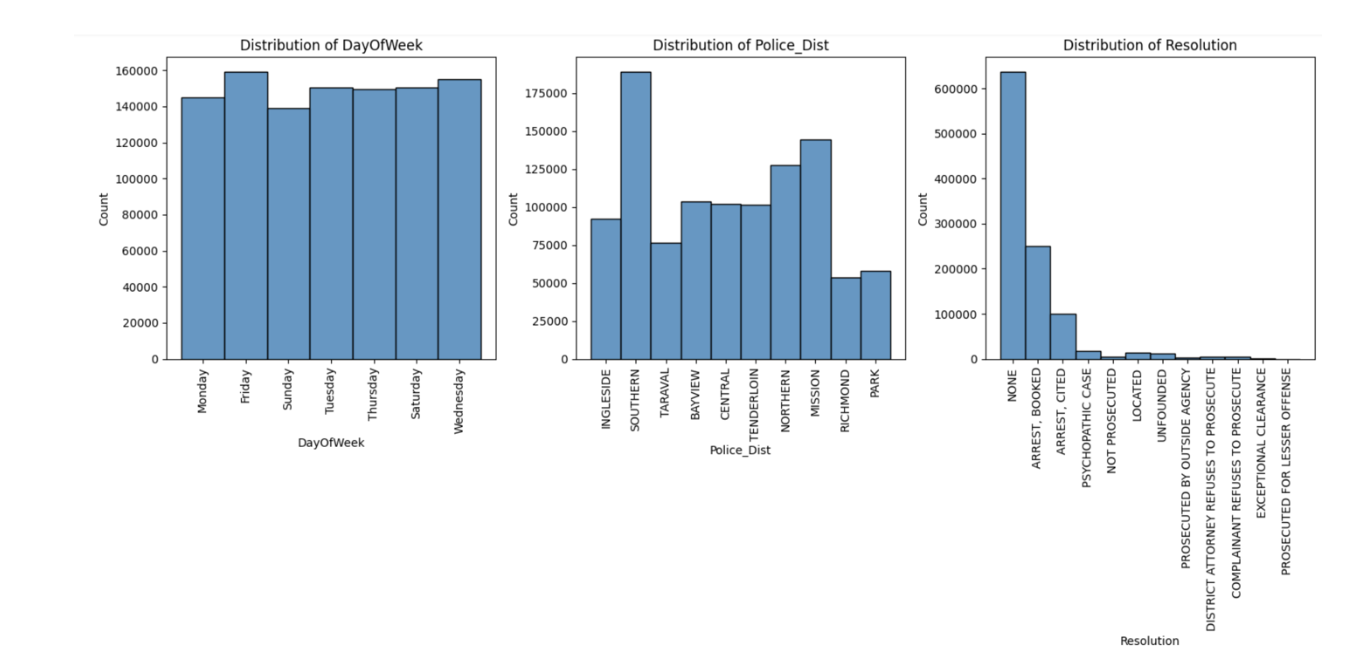
\includegraphics[width=0.5\linewidth]{img/fig1} 

}

\caption{Crime analysis based on Day of week, Police District and its resolution}\label{fig:unnamed-chunk-1}
\end{figure}

\begin{figure}

{\centering 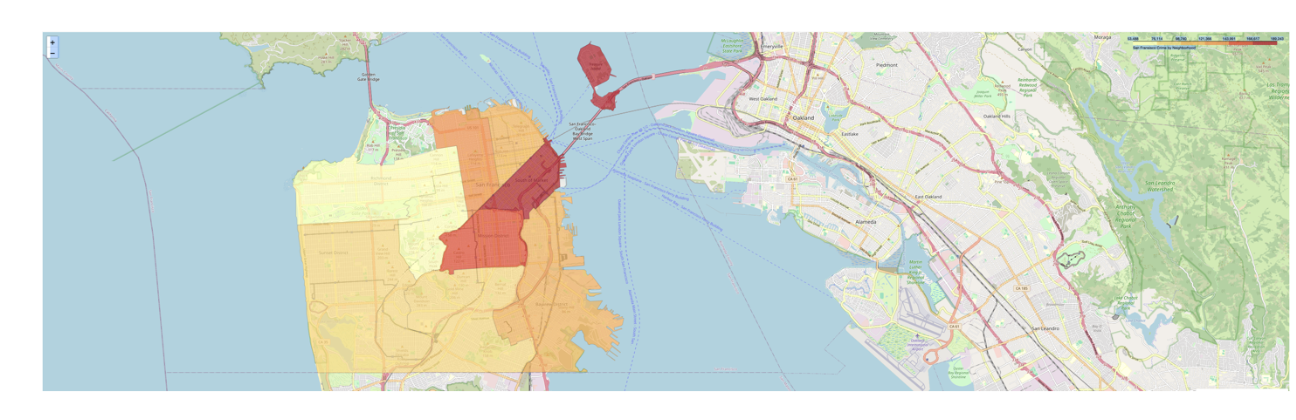
\includegraphics[width=0.5\linewidth]{img/fig2} 

}

\caption{High number of incidents concentrated in the mission district of San Francisco}\label{fig:unnamed-chunk-2}
\end{figure}

\begin{figure}

{\centering 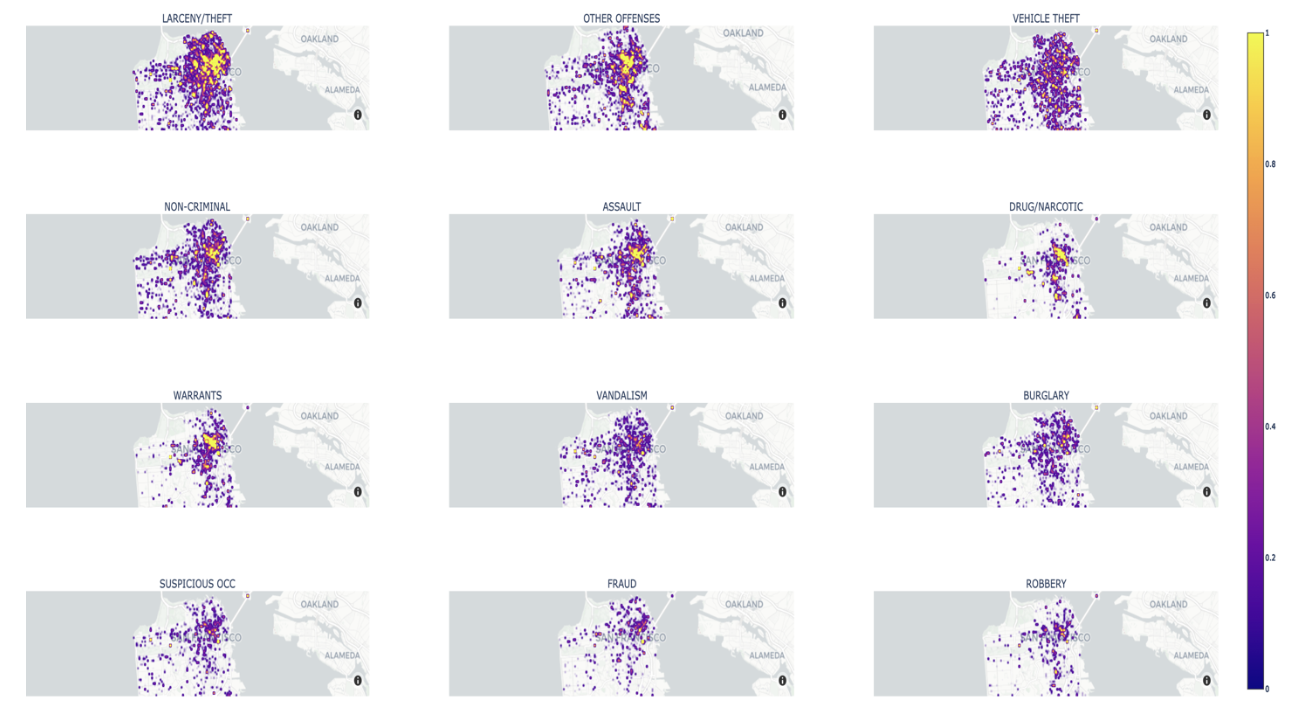
\includegraphics[width=0.9\linewidth]{img/fig3} 

}

\caption{High density of different incident categories}\label{fig:unnamed-chunk-3}
\end{figure}

\begin{figure}

{\centering 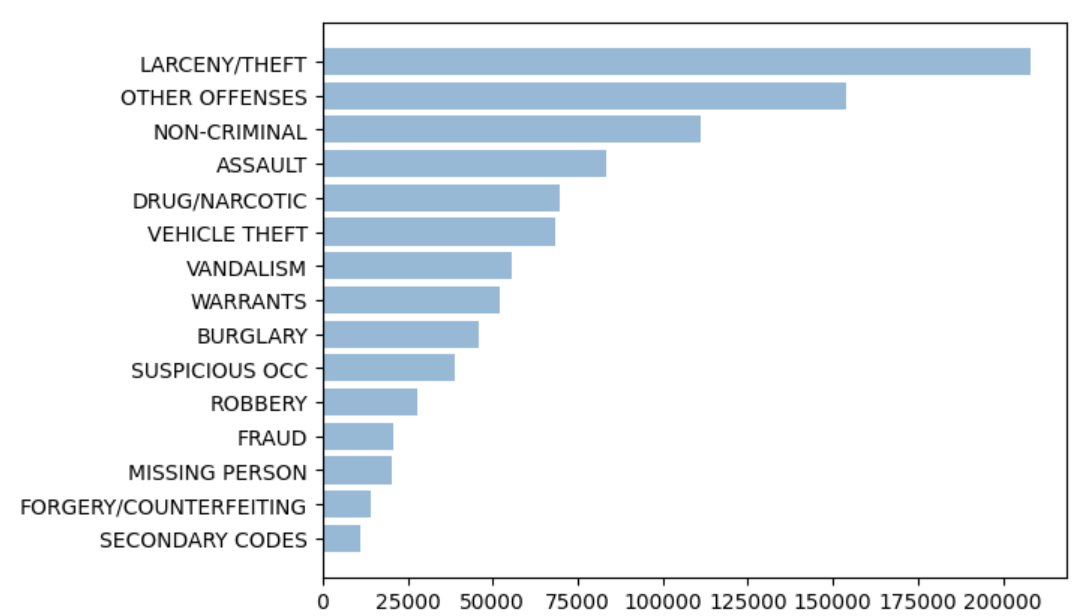
\includegraphics[width=0.7\linewidth]{img/fig4} 

}

\caption{Top incident categories}\label{fig:unnamed-chunk-4}
\end{figure}

Figure 5 shows the heat map of incidents based on the weekdays and
brighter represents the hotspots of the categories. Figure 6 shows the
heatmap of incidents based on the time of the day. Most of the crimes
are happening in the afternoon and evening hours. Figure 7 represents
the heat map representation based on the season. It shows spring and
autumn are favorable for crime cases.

\begin{figure}

{\centering 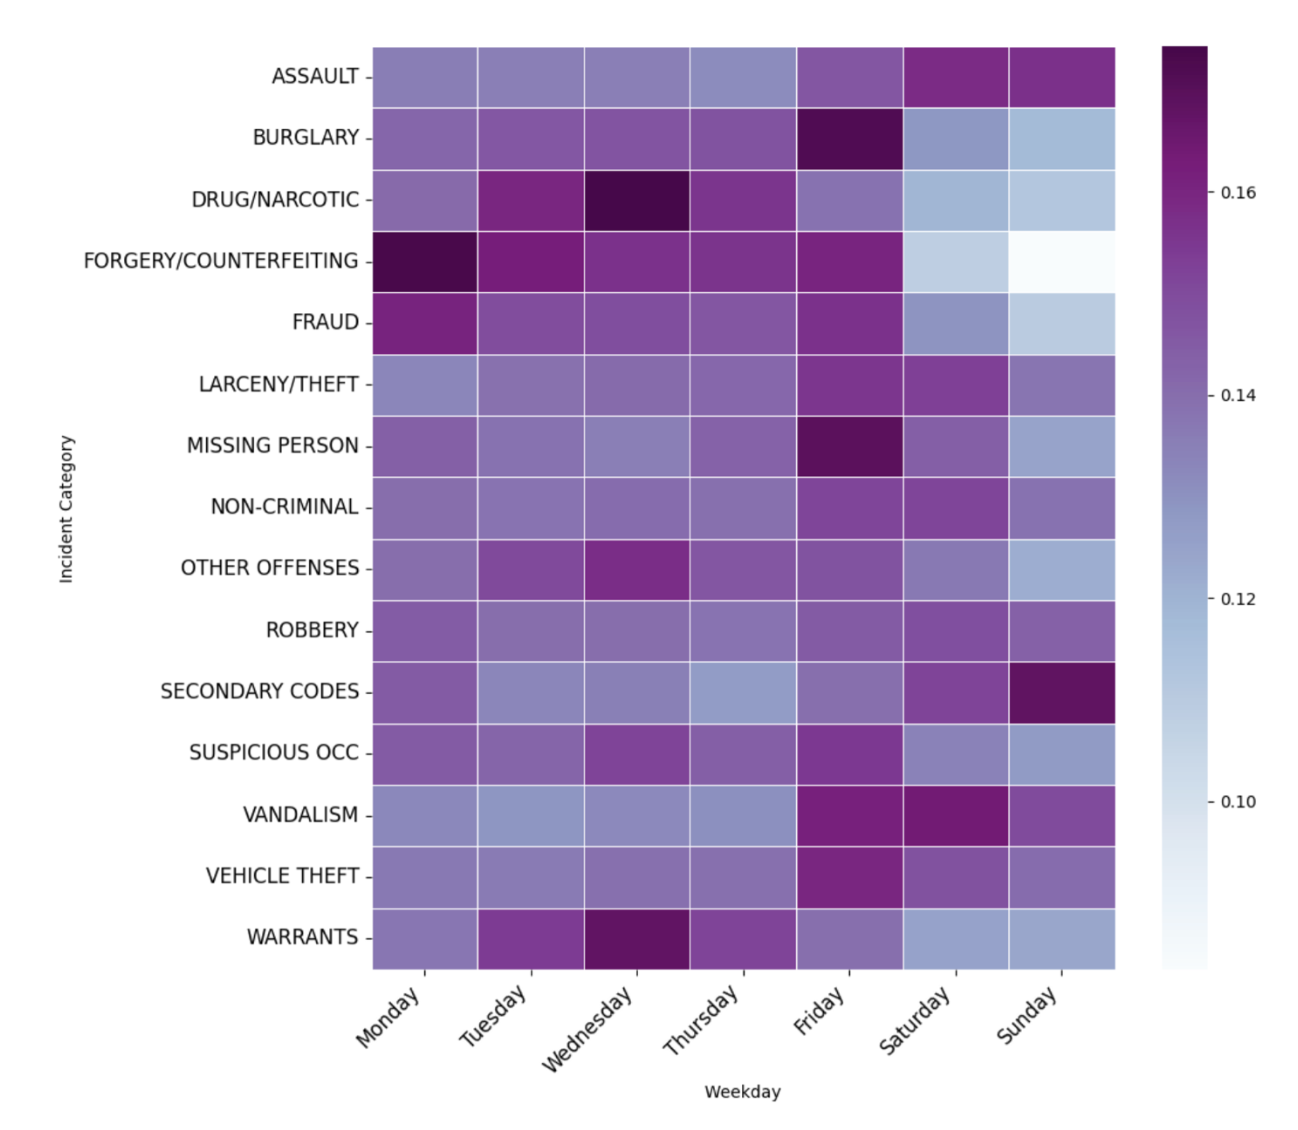
\includegraphics[width=0.7\linewidth]{img/fig5} 

}

\caption{Incidents heat map based on the day of the week}\label{fig:unnamed-chunk-5}
\end{figure}

\begin{figure}

{\centering 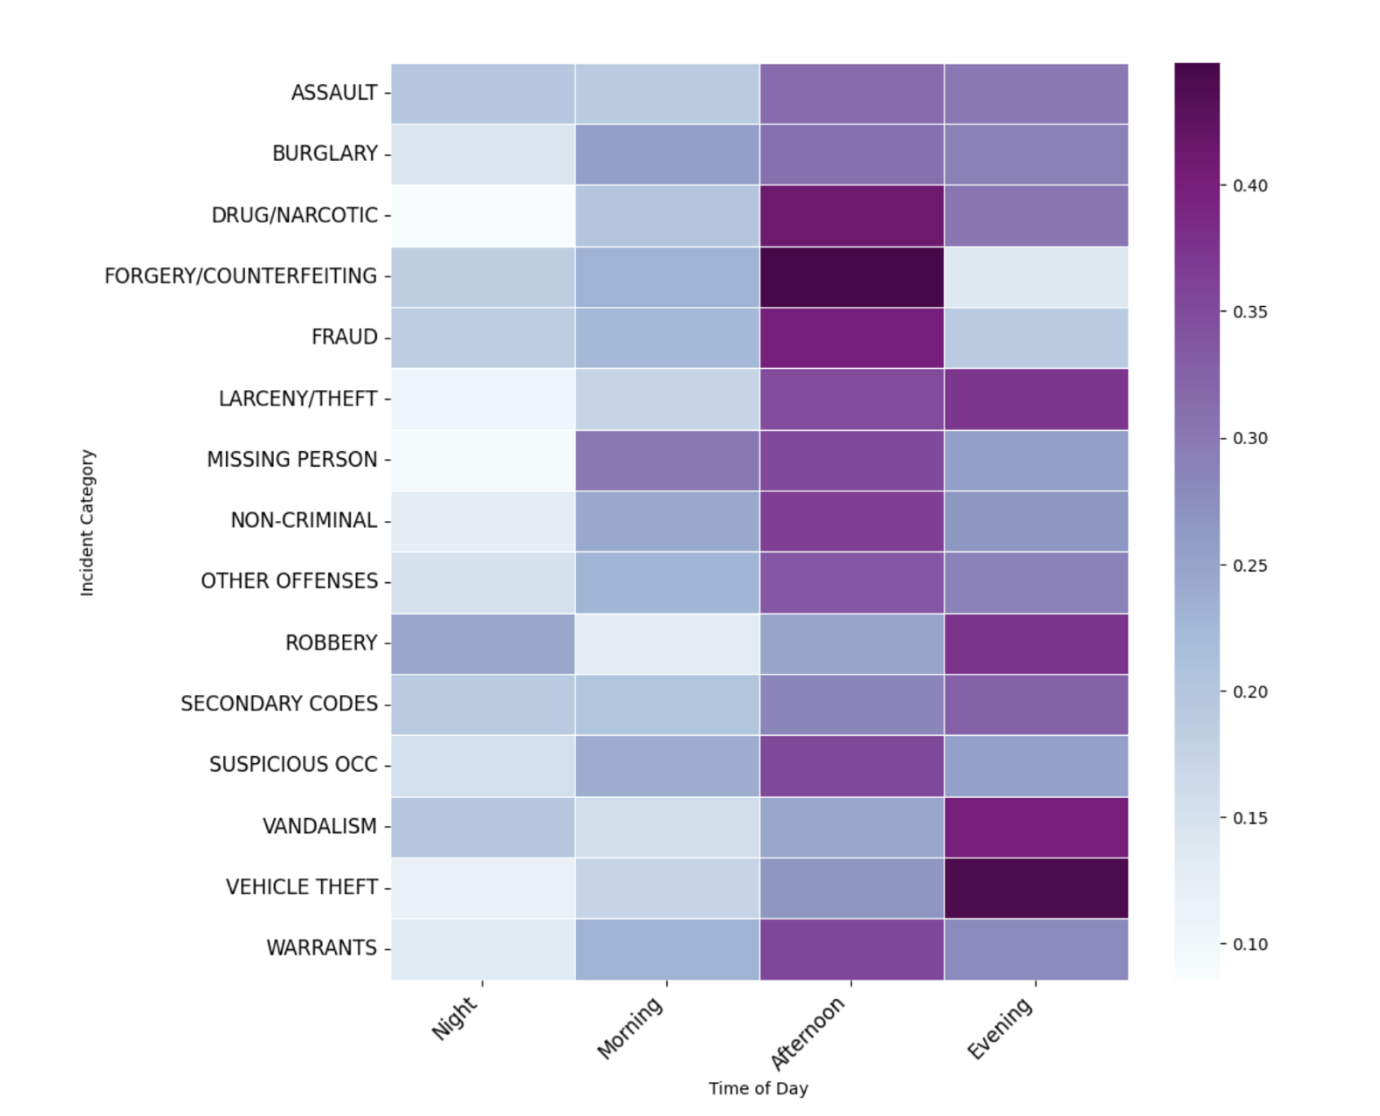
\includegraphics[width=0.7\linewidth]{img/fig6} 

}

\caption{Incidents heat map based on the time of day}\label{fig:unnamed-chunk-6}
\end{figure}

\begin{figure}

{\centering 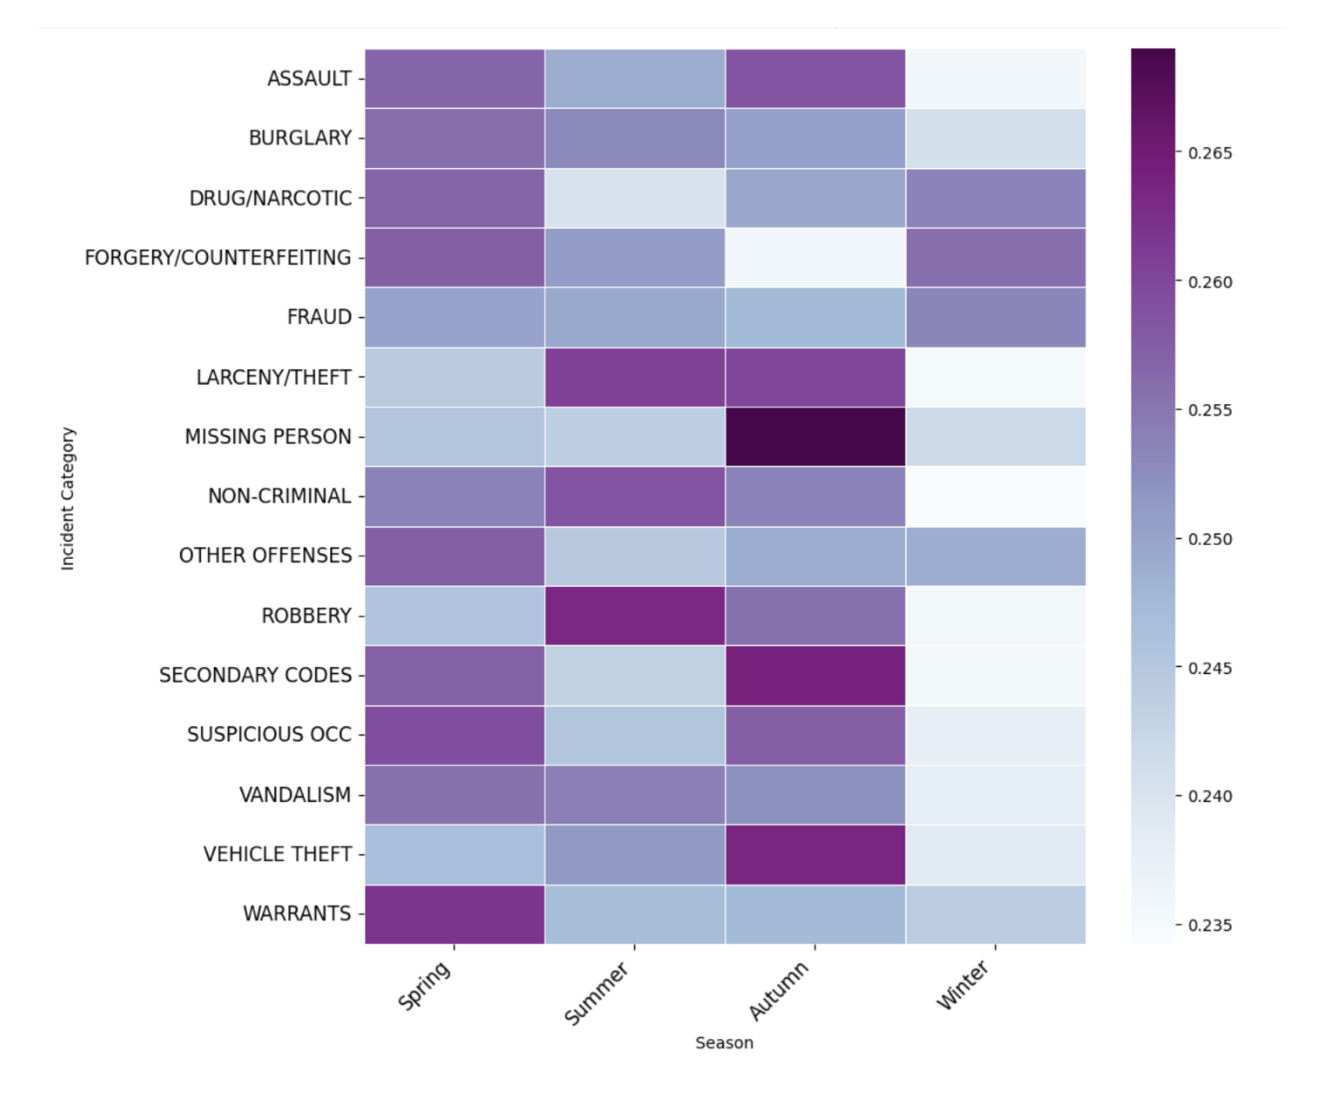
\includegraphics[width=0.7\linewidth]{img/fig7} 

}

\caption{Incidents heat map based on the time of day}\label{fig:unnamed-chunk-7}
\end{figure}

Figure 8 shows the attribute analysis based on the correlation between
them. The scale from 0 to 1 indicates the correlation and higher the
value closer to the relation of the attributes. Figure 9 shows the
number of crimes on specific days of the week. It shows crime
occurrences every Sunday. The count has reached 300 on specific Sunday
in a year and the minimum crime count on Sunday is 200.

\begin{figure}

{\centering 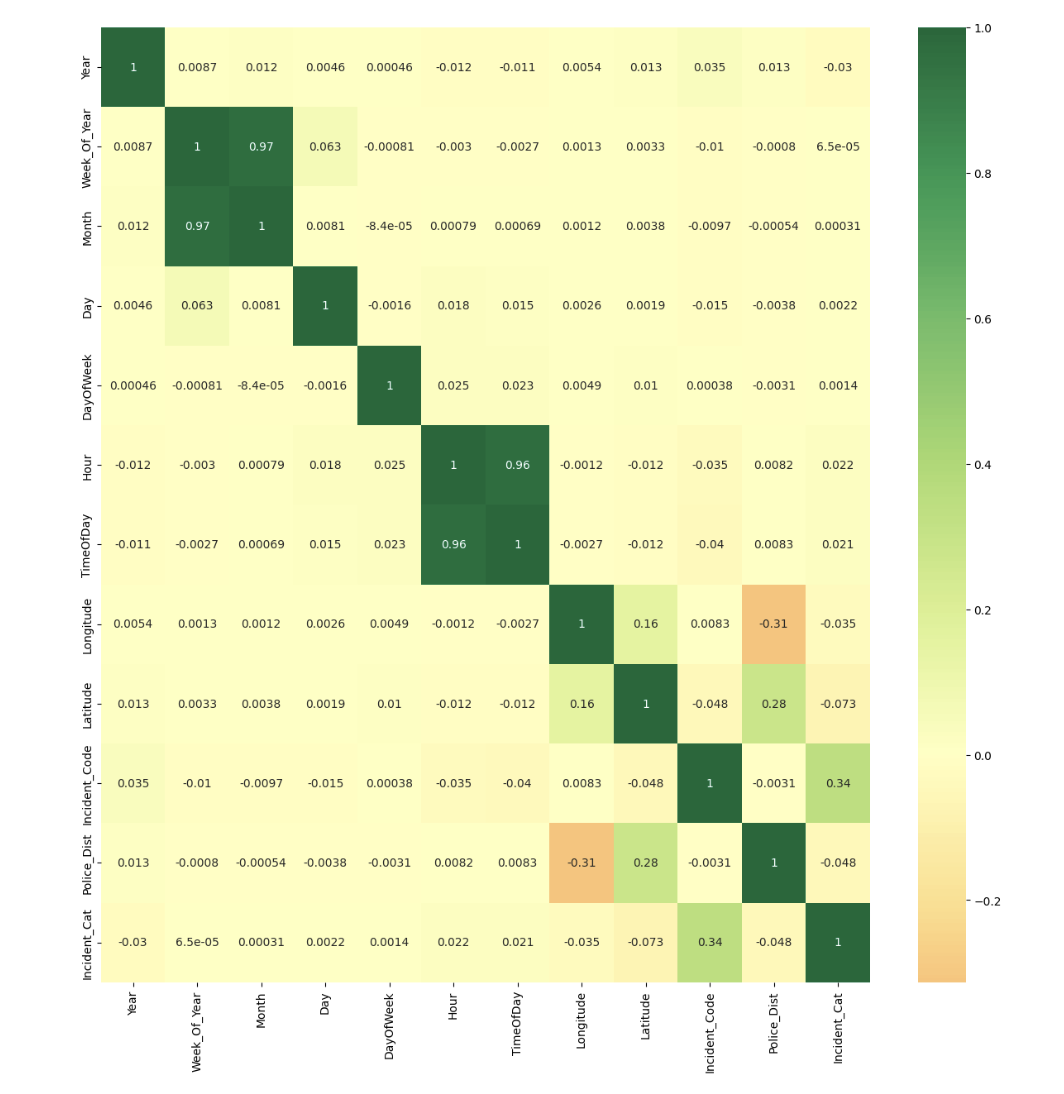
\includegraphics[width=0.9\linewidth]{img/fig8} 

}

\caption{Correlation analysis of different factors}\label{fig:unnamed-chunk-8}
\end{figure}

\begin{figure}

{\centering 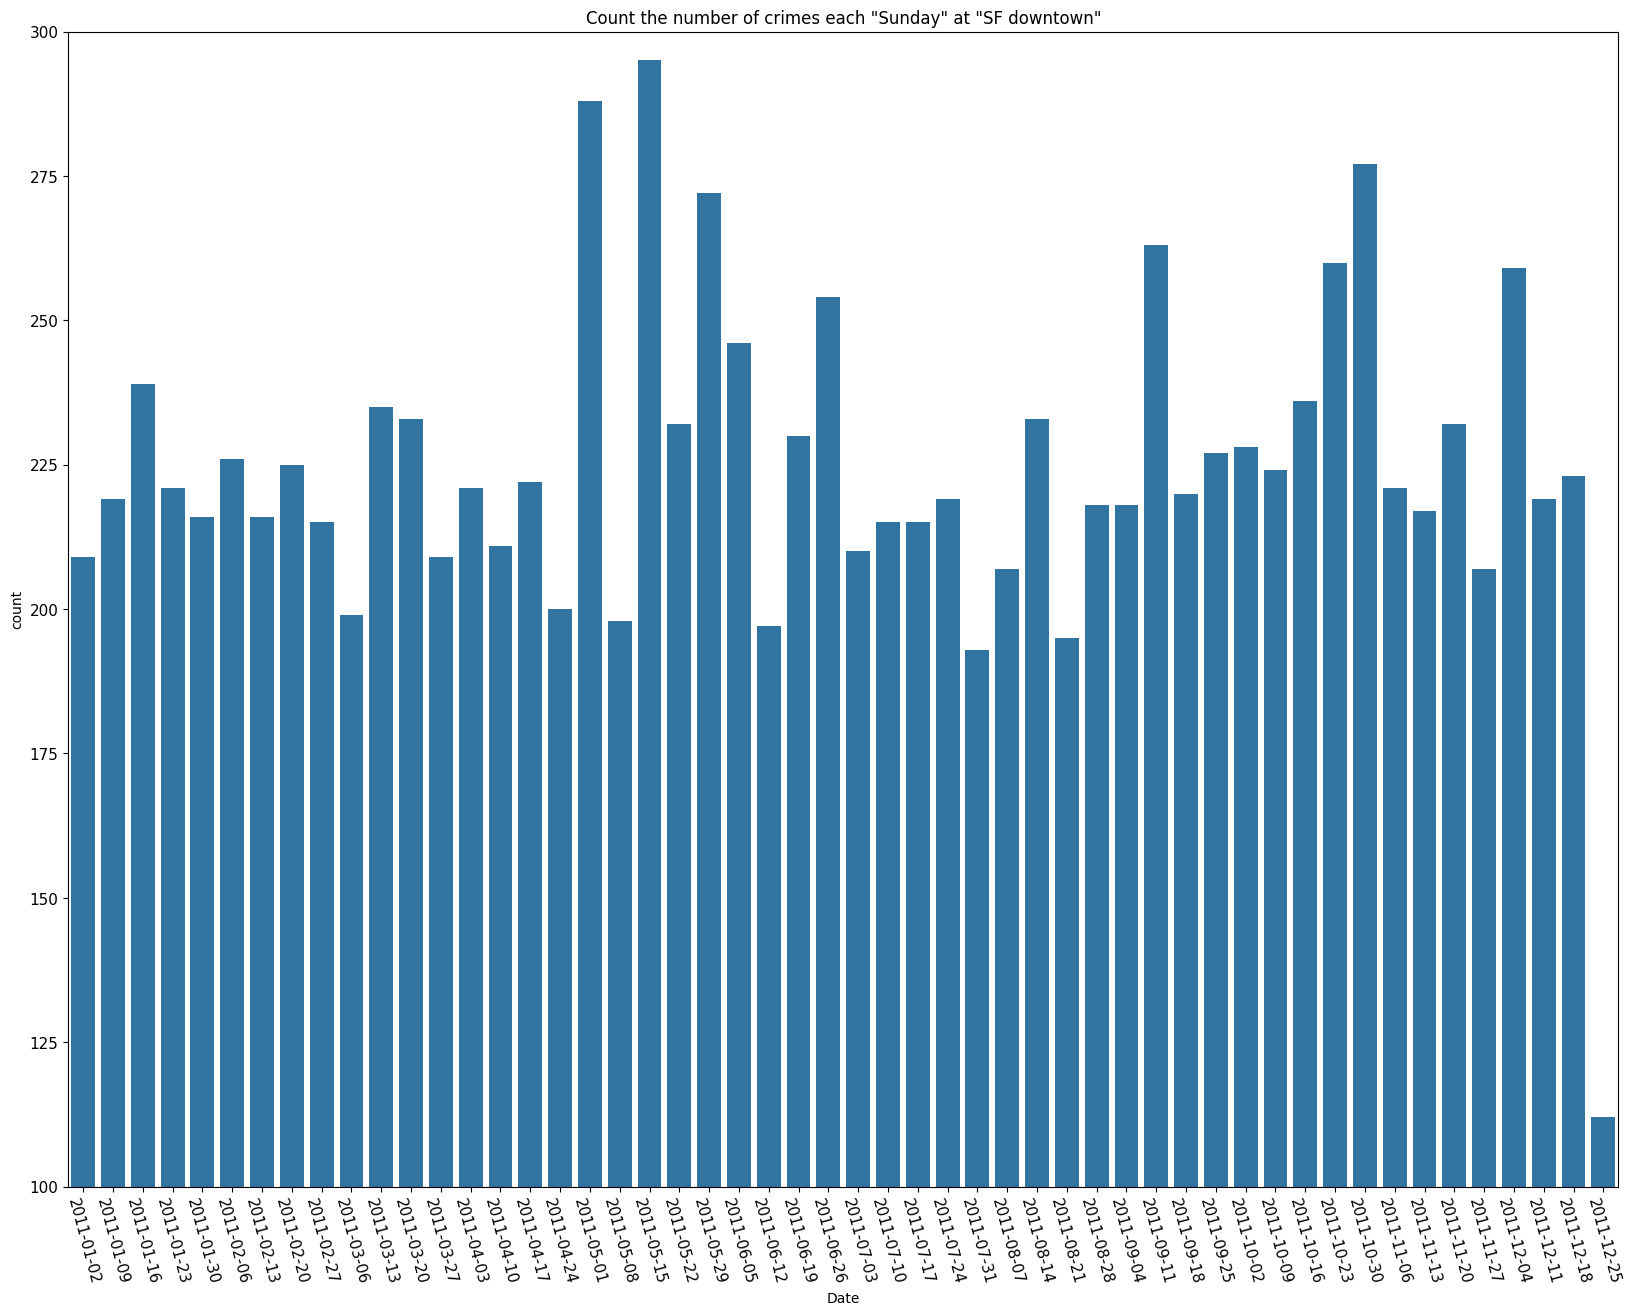
\includegraphics[width=0.8\linewidth]{img/fig9} 

}

\caption{Number of crimes occurred on Sunday basis}\label{fig:unnamed-chunk-9}
\end{figure}

\begin{figure}

{\centering 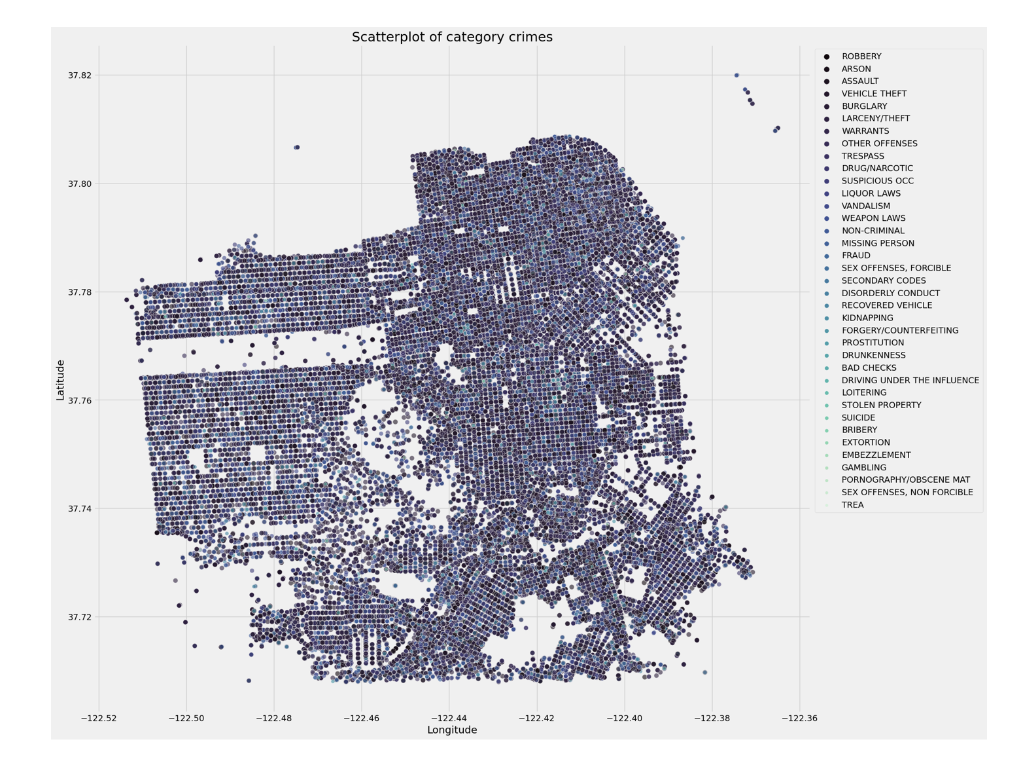
\includegraphics[width=0.7\linewidth]{img/fig10} 

}

\caption{Top crimes occurred based on the map}\label{fig:unnamed-chunk-10}
\end{figure}

\begin{figure}

{\centering 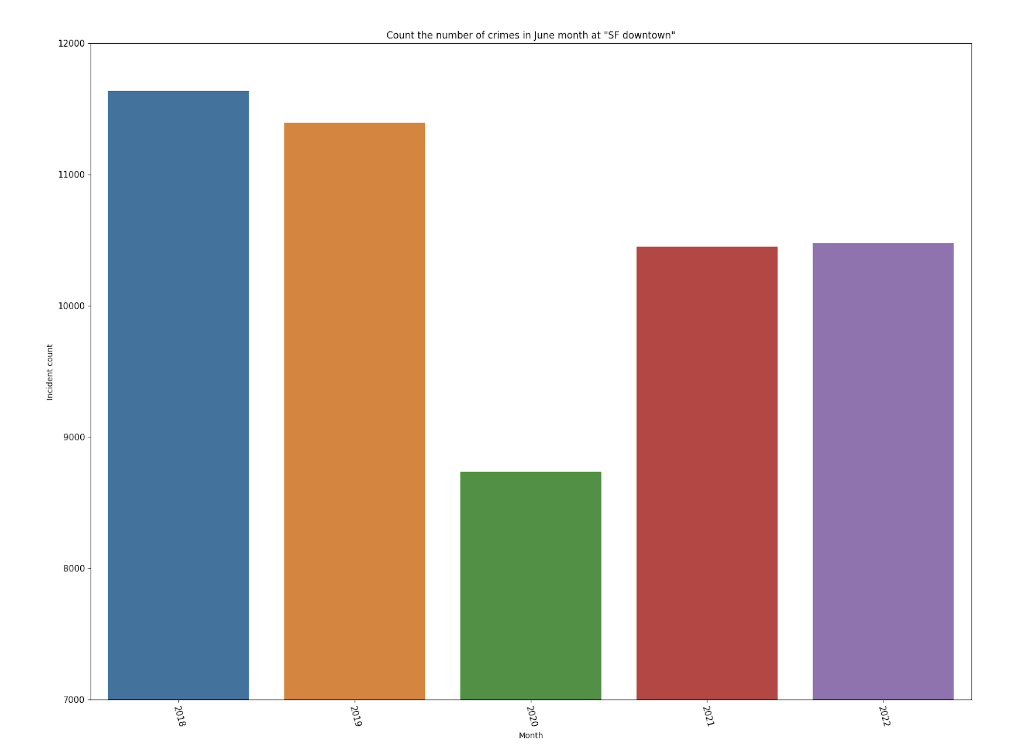
\includegraphics[width=0.5\linewidth]{img/fig11} 

}

\caption{Crime count based on the year}\label{fig:unnamed-chunk-11}
\end{figure}

Figure 10 shows the scatter plot of Top crimes across the San Francisco
region. The seasons like summer and fall are attracting more crimes. The
analysis clearly shows that the number of crimes had decreased during
2020, it might be because of the Pandemic. The crimes are mostly occurring
during afternoon hours, and few are happening during evening hours. If
we analyze the yearly trends, the occurrence of the crimes has changed
from fall to winter after the pandemic. The attributes timeofday, hour,
latitude, longitude, and police distinct are highly correlated
attributes. Analysis of historical data from 2003 to 2018 gives more
meaningful insights on the data pattern, trend and how to build the
model.

The data of San Francisco from the year 2018 onwards shows quite
deviation as follows.

\begin{itemize}
\tightlist
\item
  The number of crime categories have increased.
\item
  Theft is the highest number of crimes that has been occurring
  continuously.
\item
  Missing people crimes have dominated in recent years.
\item
  It looks like the middle of the week which is Wednesday is tagged to
  Drug offense.
\item
  Crime count has increased in proportion to population growth.
\item
  Crimes more often occurring in the afternoon and pushing towards
  evening hours.
\item
  More crimes that were occuring during winter in early 2018 has shifted
  to other seasons making winter quite non-crime seasons in the recent
  years.
\end{itemize}

The analysis drives the use of different models like Random Forest,
K-nearest neighbor, ANN, Tablet and time series analysis are created to
understand the behavior of the data with the model.

\section{Methods}\label{methods}

\textbf This project is intended to be used for
crime applications, such as assistance for the crime victims, police
department, Victim service division, crime map and public safety
awareness, Crime rates and statistics, Attorney, and legal advocacy. It
is particularly intended for public safety awareness.

Random Forest: Random Forest is an ensemble supervised machine learning
algorithm for classification and regression problems. It involves
building multiple decision trees on different samples and aggregating
the predictions using a majority vote for classification.

The k-nearest neighbors (KNN) algorithm is a type of supervised machine
learning algorithm used to solve classification. The algorithm estimates
the likelihood that a data point will become a member of one group or
another based on what group the data points nearest to it belong to. It
is a non-parametric algorithm since it is robust to underlying
distributions of the data.

Artificial neural networks are human brain cells inspired systems which
are intended to replicate the way that humans learn. Neural networks
consist of input and output layers, as well as (in most cases) a hidden
layer consisting of units that transform the input into something that
the output layer can be   used. ANNs have three layers that are interconnected
and consist of neurons. The first layer sends data to the second layer,
which in turn sends the next output to the third layer. ANNs are
considered non-linear statistical data modeling tools where the complex
relationships between inputs and outputs are modeled or patterns are
found.

TabNet is a deep tabular data learning architecture and one of the first
transformer based models that uses sequential attention to choose which
features to reason from at each decision step. The TabNet encoder is
composed of a feature transformer, an attentive transformer and feature
masking. A split block divides the processed representation to be used
by the attentive transformer of the subsequent step as well as for the
overall output. For each step, the feature selection mask provides
interpretable information about the model's functionality, and the masks
can be aggregated to obtain global feature important attribution. The
TabNet decoder is composed of a feature transformer block at each step.

In the feature transformer block, a 4-layer network is used, where 2 are
shared across all decision steps and 2 are decision step-dependent. Each
layer is composed of a fully-connected (FC) layer, BN and GLU
nonlinearity. An attentive transformer block is a single layer mapping
modulated with a prior scale information which aggregates how much each
feature has been used before the current decision step. sparsemax is
used for normalization of the coefficients, resulting in sparse
selection of the salient features. There are different parameters for
fine tuning the model for better performance. The parameters like
learning rate, epochs, decay rate, patience and batch size gives better
control of the models. Some of the initial methods followed in the paper
are

The learning rate is initially set to, lr = 0.020

After 20 epochs, a decay rate of 0.95 will be applied The result is
simply the product of our learning rate and decay rate 0.02*0.95 then we fit the model to our data. Basically it says the
train and validation sets will be evaluated for a total of 30 iterations
(epochs). The patience parameter shows the improvement in
metrics is not observed after 30 consecutive epochs help to get the best weights. The
batch size of 10000 was selected based on recommendations from TabNet's
paper, where they suggest a batch size of up to 10\% of the total data.


Since the crime pattern also has a strong time based component we also
explored time-series forecasting methods. These methods consider the
history along with current data to forecast values through its trends over a period of
time or a specific point in the future. Using time series models
it is good to forecast the number of crimes that occur in the future.
This can be drilled down further up to different category predictions.

\section{Metrics}\label{metrics}

Evaluation metrics include confusion metrics that contain the values of
True positive, , False Positive, True Negative and False Negative that
helps in False Positive rate and False Negative rate to measure
disproportionate model performance errors. The fraction of negative (not
falling to the same category) and positive (same category) predictions
that are incorrectly predicted to be positive and negative,
respectively, are also reported. These metrics provide values for
different errors that can be calculated and provide better understanding
of classification. The accuracy of the models is between 83 -- 98 \%
achieved through different ML and AI approaches. All metrics reported at
the .2 decision threshold.

\begin{figure}

{\centering 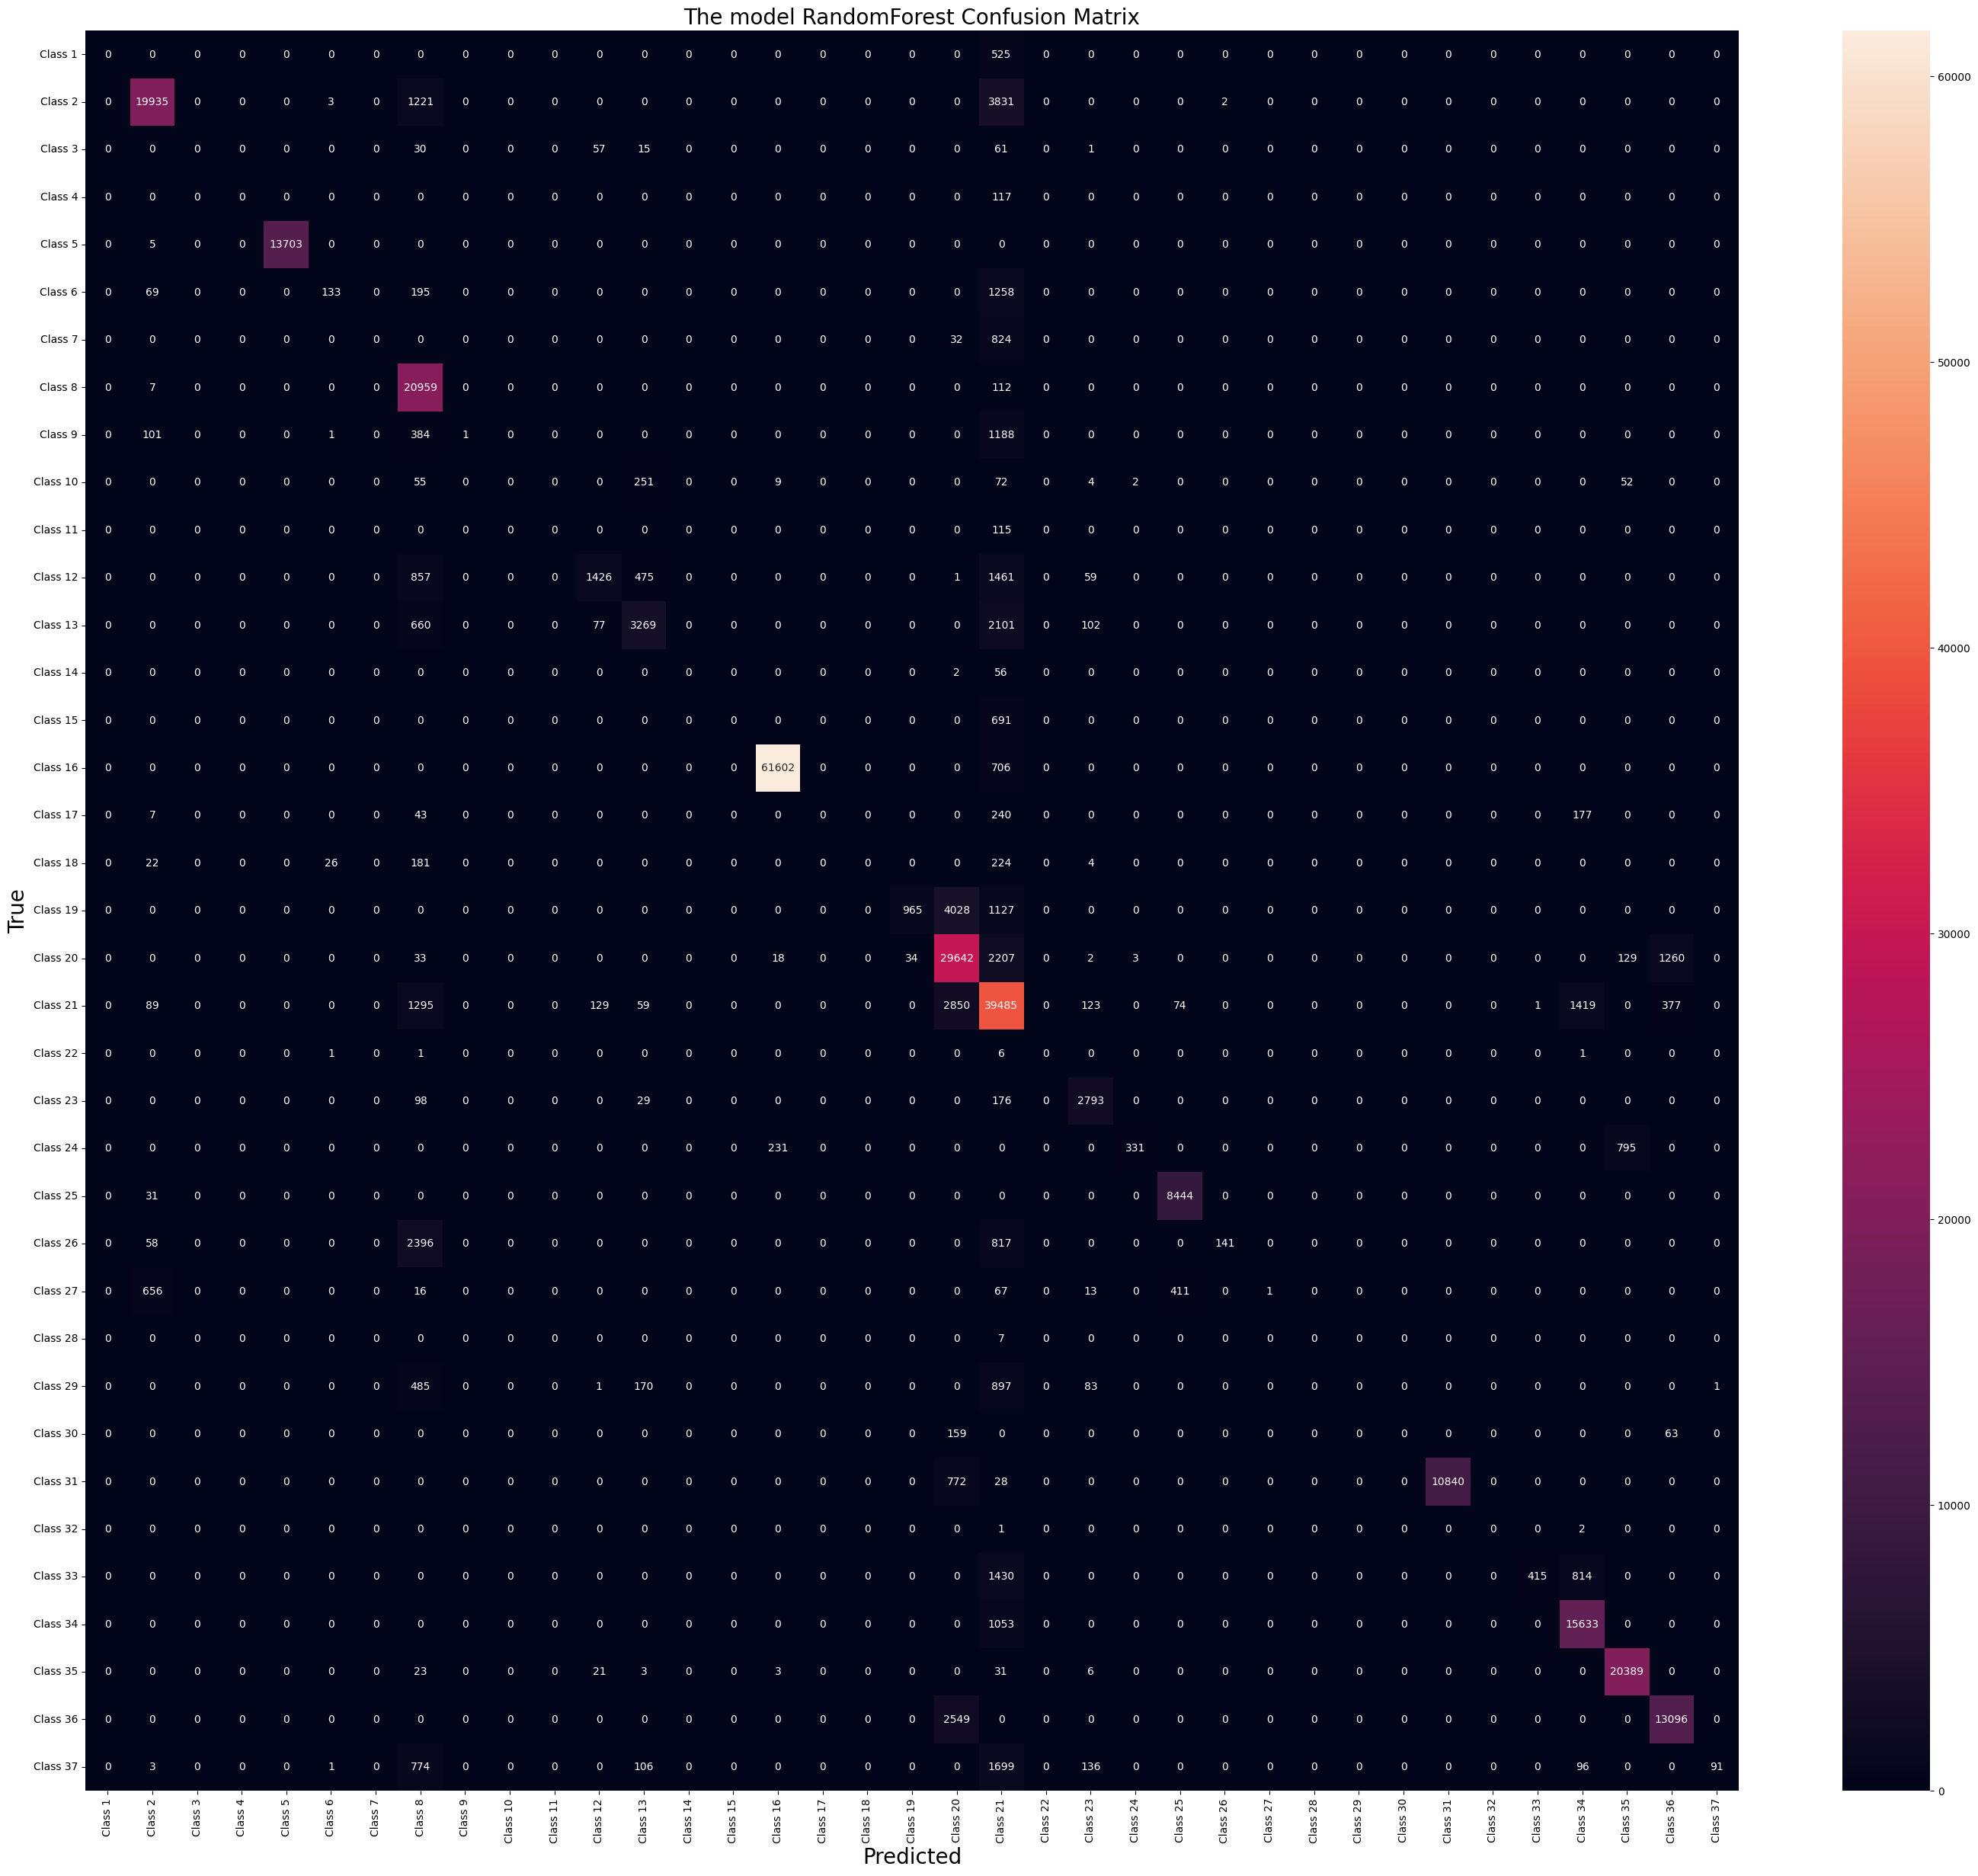
\includegraphics[width=0.7\linewidth]{img/fig12} 

}

\caption{Confusion metrics for Random Forest}\label{fig:unnamed-chunk-12}
\end{figure}

\begin{figure}

{\centering 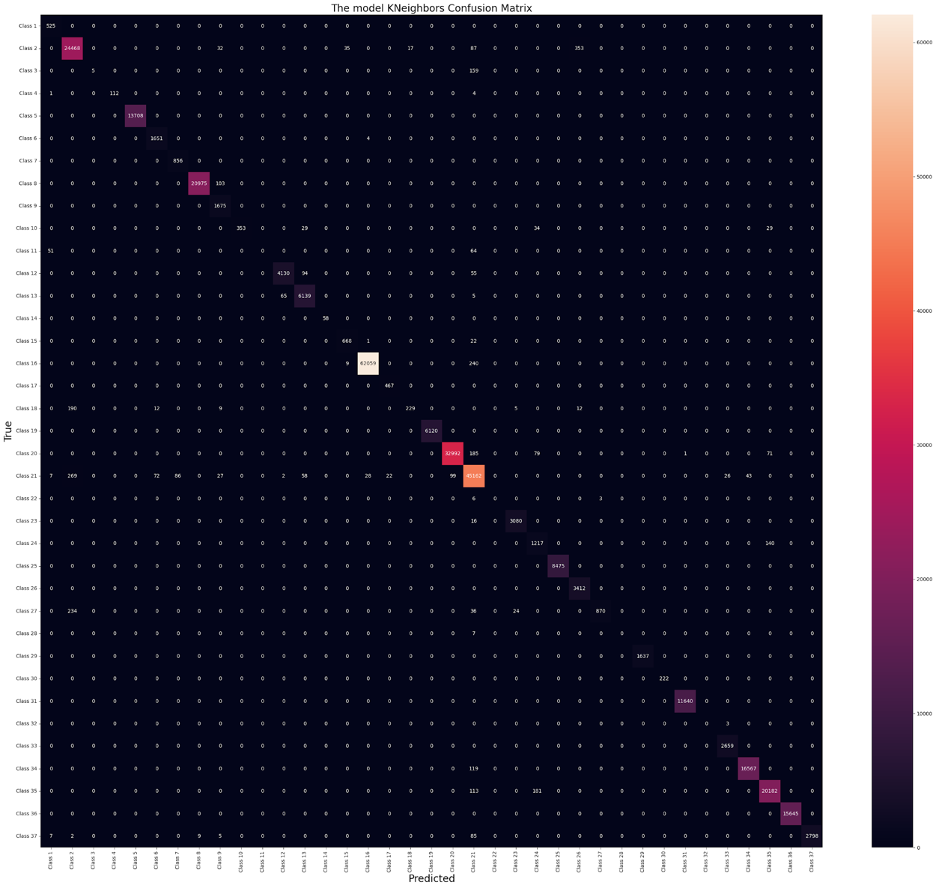
\includegraphics[width=0.7\linewidth]{img/fig13} 

}

\caption{Confusion metrics for K-Nearest Neighbor.}\label{fig:unnamed-chunk-13}
\end{figure}

\begin{figure}

{\centering 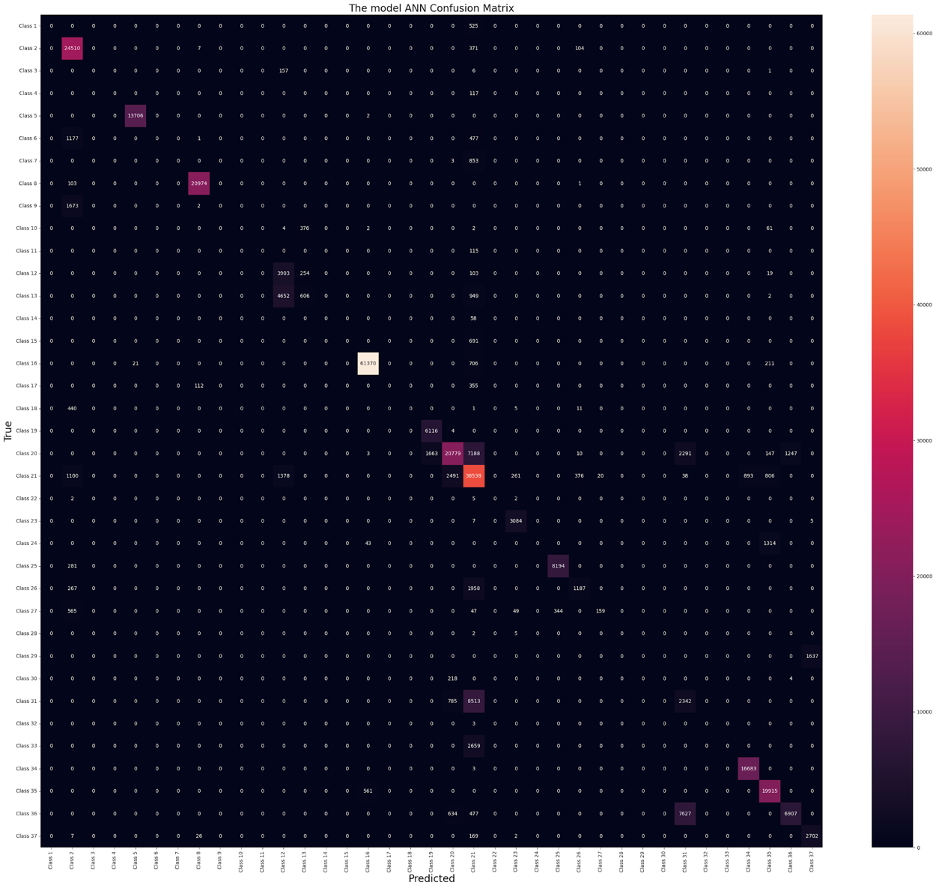
\includegraphics[width=0.7\linewidth]{img/ANN} 

}

\caption{Confusion metrics for Artificial Neural Network.}\label{fig:unnamed-chunk-13b}
\end{figure}

\begin{figure}

{\centering 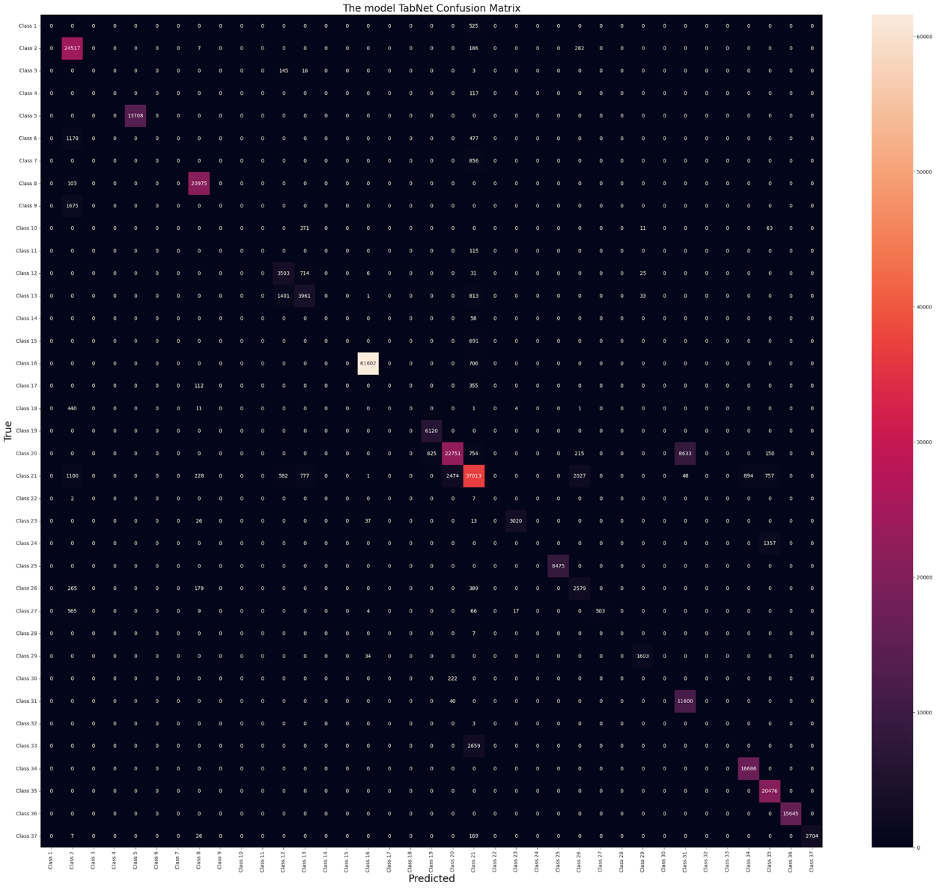
\includegraphics[width=0.7\linewidth]{img/TabNet} 

}

\caption{Confusion metrics for TabNet.}\label{fig:unnamed-chunk-13c}
\end{figure}

\section{Discussion and Impact}\label{discussion-and-impact}

We always approach ML algorithms for classification problems, but Deep
learning models and TabNet are also good for classification problems on
tabular data. To build the model's hyperparameter and different features
are important factors for the algorithm. In the case of RandomForest
using entropy criterion gives better accuracy than Gini Criterion. The
number of estimators in K nearest neighbor plays a significant role in
the algorithm. In ANN deep neural network architecture, activation,
optimizer, and loss should be carefully chosen to get better
performance. Learning, decay rate and batch size plays a major role in
TabNet. Time series depends on how data is closely related to the
previous trends. It is a good practice to keep a smaller number of
classes or grouping similar classes as one to get better accuracy. High
amount of data helps in fine tuning the model. Uniqueness and data
consistency are important factors to build the model. If we build
different models it provides more confidence and ideas to weigh to
choose the model for prediction.

\section{Evaluation and Reflection}\label{evaluation-and-reflection}

Metrics like accuracy provides the confidence to identify the better performance
of the model. Confusion matrix helps in visual representation of the prediction
and its deviation. Classification reports provide the different metrics
like precision, recall, f1-score for different classes of the categories. This
gives better pictures on how the model is good enough for each
classification. MSE and RMSE help in clear view of time series model
performance. The loss function greatly influences the performance or
accuracy of the model. Table 1 represent the accuracy of each model for different dataset
and classes respresent the number of crime categories of the given data.

\begin{table}[ht]
\centering
\begin{tabular}{|c|c|c|c|c|}
\hline
Model & SFO(2003-2018) & SFO(2018- 2022) & Boston(2022)\\ \hline
Random Forest & 83.70 \% & 89.27 \% & 78.69 \% \\ \hline
K Neighbour   & 98.79 \% & 98.59 \% & 72.70 \% \\ \hline
ANN           & 86.07 \% & 81.63 \% & 55.58 \% \\ \hline
TabNet        & 89.25 \% & 86.29 \% & 63.53 \% \\ \hline
Time Series   & 37.33 \% & 42.56 \% & 26.89 \% \\ \hline
Classes & 37 & 50 & 120 \\ \hline
\end{tabular}
\vspace{10pt}
\caption{Comparison of Machine and Deep learning models}
\label{tab:example_table}
\end{table}

\section{Application}\label{application}

To create the web application (henceforth referred as webapp) start with
YAML code as the first line of the jupyter notebook by providing the
required filters as part of the code. Define the dashboard name as part
of the WebAPP page. The webapp needs the mercury libraries hence install
the libraries for python and use the command such as jupyter trust,
mercury add, and mercury watch on the created file. This will initiate
the webapp in the link ``http://127.0.0.1:8000'' .

\begin{figure}

{\centering 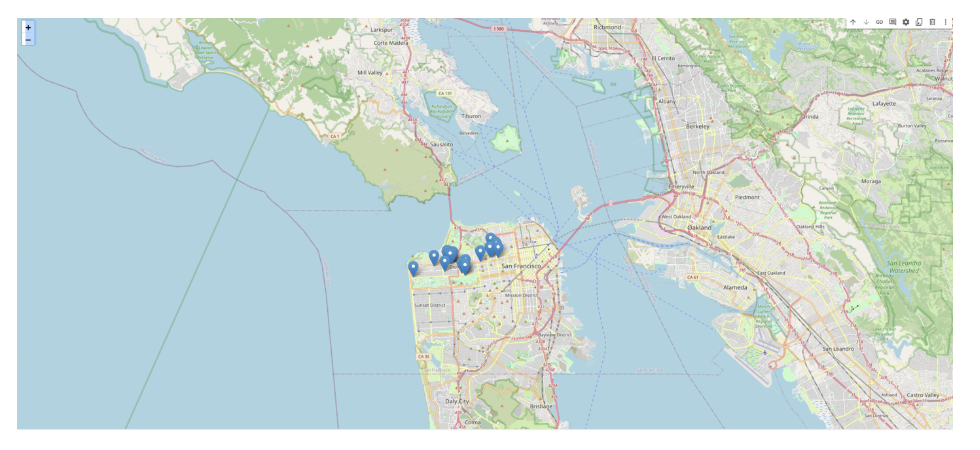
\includegraphics[width=0.5\linewidth]{img/fig14a} 

}

\caption{Webapp to identify the location and incidents}\label{fig:unnamed-chunk-13}
\end{figure}

\subsection{Interactive Dashboard}\label{interactive-dashboard}

The interactive dashboard needs different python libraries for map and
interactive display and methods. The folium library is used for the map display
and ipywidgets library for interactive display are installed for python.
The next step is to identify the important features for the dashboard
and followed by initialization of the widgets for the features that are
part of filter conditions. The description and layout specify the
display of the filter in specific format. The function should be defined
to get the data and transform the data if necessary to required
aggregation. Use folium method to display map and any other graph or
chart if necessary. Use widget interactive method to invoke the function
and required widget that are part of filters to display the interactive
dashboard.

\begin{figure}

{\centering 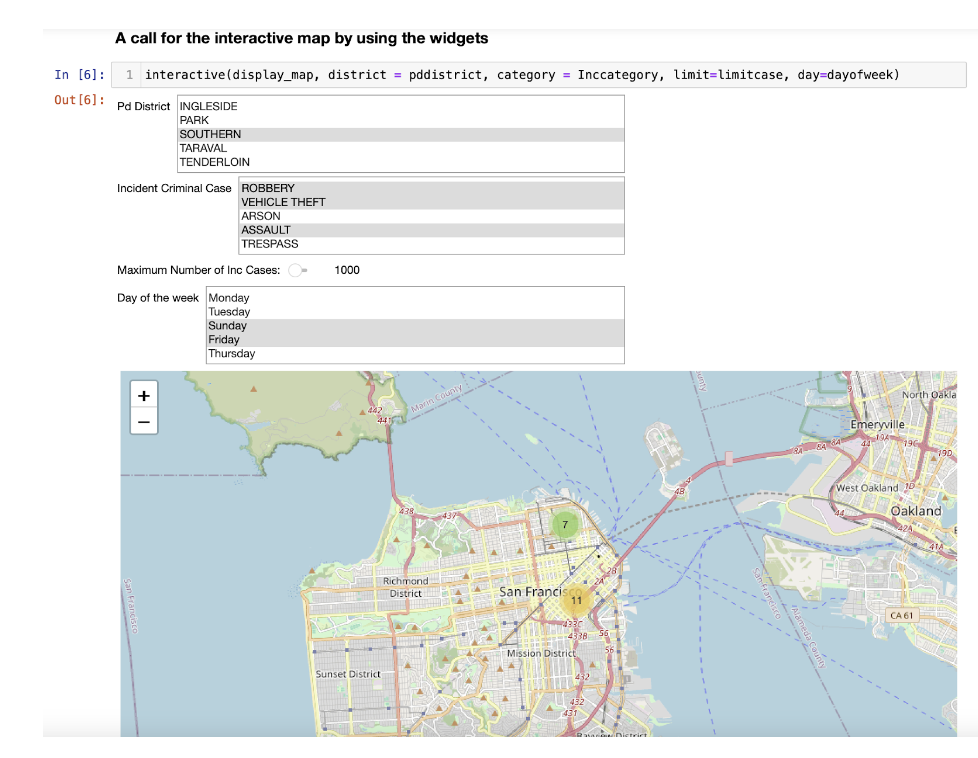
\includegraphics[width=0.5\linewidth]{img/fig14b} 

}

\caption{Interactive map to facilitate different requirements}\label{fig:unnamed-chunk-14}
\end{figure}

\section{Limitation}\label{limitation}

This project is to predict the incident categories. The number of
categories may vary based on the data. It is not suitable for
identification of person or thing responsible for crime; Crimes were
categorized based on evidence produced and justified report. It is
difficult to get the census data based on city and geographical
location.

\section{Conclusion and Future Work}\label{conclusion-and-future-work}

We always tend to move towards ML algorithms for classification problems
as it is white box, but there are other models like deep learning, time
series and TabNet which can better fit and are easy to implement. Even
Though ML algorithms overcome the Deep learning and TabNet models, more
data and fine tuning of any models perform better for the given data.
This paper presents the performance and comparison of Machine learning
and deep learning models. It also includes the different methods like
TabNet and includes effective interactive dashboard creation and webapp
applications. The method is applied to different datasets to explain the
flexibility of the approach used. The random forest comparison was done
using both gini and entropy criteria, weighted K-nearest neighbor using
100 estimators. A deep tabular data learning called TabNet that uses
sequential attention mechanisms and a more effective fine-tuning
approach is used. Each model is compared across the confusion matrix and
classification report. This project deals with all the methods using
python to make the users more friendly and reduce infrastructure cost.
It is easy to use the same method to any crime dataset with little
modification to the given data to fit to the required format and
attributes. Webapp and interactive map gives friendly and better
visualization of the data. The crimes are concentrated towards the
particular place, and it might be tagged to population or poverty.
Direction of the feature work is to get the census data based on city
and geographical location to link the crime to specific location and its
cause by considering population, social status and education.

\section*{References}\label{references}
\addcontentsline{toc}{section}{References}

\phantomsection\label{refs}
\begin{CSLReferences}{1}{0}
\bibitem[\citeproctext]{ref-brantingham2010nodes}
Brantingham, PL, and PJ Brantingham. 2010. {``Nodes, Paths, and Edges:
Considerations on the Complexity of Crime and the Physical Environment
(1993).''} In \emph{Classics in Environmental Criminology}, 289--326.
Routledge.

\bibitem[\citeproctext]{ref-darshan2022crime}
Darshan, MS, and Shankaraiah Shankaraiah. 2022. {``Crime Analysis and
Prediction Using Machine Learning Algorithms.''} In \emph{2022 IEEE 2nd
Mysore Sub Section International Conference (MysuruCon)}, 1--7. IEEE.


\bibitem[\citeproctext]{ref-ghushami2022crime}
A. H. Al-Ghushami, D. Syed, J. Sessa and A. Zainab. 2022. 
{``CIntelligent Automation of Crime Prediction using Data Mining.''} 
In \emph{2022 IEEE 31st International Symposium on Industrial Electronics (ISIE), Anchorage, AK, USA}

\bibitem[\citeproctext]{ref-gahalot2020crime}
Gahalot, Akanksha, Suraina Dhiman, Lokesh Chouhan, et al. 2020. {``Crime
Prediction and Analysis.''} In \emph{2nd International Conference on
Data, Engineering and Applications (IDEA)}, 1--6. IEEE.

\bibitem[\citeproctext]{ref-menaka2022analysis}
Menaka, M, and B Booba. 2022. {``Analysis to Improve Classifier Accuracy
in Crime Data Prediction.''} In \emph{2022 6th International Conference
on Computing Methodologies and Communication (ICCMC)}, 721--25. IEEE.

\bibitem[\citeproctext]{ref-pandya2022analysis}
Pandya, Darshanaben Dipakkumar, Geetanjali Amarawat, Abhijeetsinh
Jadeja, Sheshang Degadwala, and Dhairya Vyas. 2022. {``Analysis and
Prediction of Location Based Criminal Behaviors Through Machine
Learning.''} In \emph{2022 International Conference on Edge Computing
and Applications (ICECAA)}, 1324--32. IEEE.

\bibitem[\citeproctext]{ref-rossmo1999geographic}
Rossmo, D Kim. 1999. \emph{Geographic Profiling}. CRC press.

\bibitem[\citeproctext]{ref-sherman1989hot}
Sherman, Lawrence W, Patrick R Gartin, and Michael E Buerger. 1989.
{``Hot Spots of Predatory Crime: Routine Activities and the Criminology
of Place.''} \emph{Criminology} 27 (1): 27--56.

\bibitem[\citeproctext]{ref-tayebi2012understanding}
Tayebi, Mohammad A, Richard Frank, and Uwe Glässer. 2012.
{``Understanding the Link Between Social and Spatial Distance in the
Crime World.''} In \emph{Proceedings of the 20th International
Conference on Advances in Geographic Information Systems}, 550--53.

\bibitem[\citeproctext]{ref-tayebi2015learning}
Tayebi, Mohammad A, Uwe Gla, Patricia L Brantingham, et al. 2015.
{``Learning Where to Inspect: Location Learning for Crime Prediction.''}
In \emph{2015 IEEE International Conference on Intelligence and Security
Informatics (ISI)}, 25--30. IEEE.

\bibitem[\citeproctext]{ref-weisburd2012criminology}
Weisburd, David, Elizabeth R Groff, and Sue-Ming Yang. 2012. \emph{The
Criminology of Place: Street Segments and Our Understanding of the Crime
Problem}. Oxford University Press.

\bibitem[\citeproctext]{ref-yadav2017crime}
Yadav, Sunil, Meet Timbadia, Ajit Yadav, Rohit Vishwakarma, and
Nikhilesh Yadav. 2017. {``Crime Pattern Detection, Analysis \&
Prediction.''} In \emph{2017 International Conference of Electronics,
Communication and Aerospace Technology (ICECA)}, 1:225--30. IEEE.

\bibitem[\citeproctext]{ref-arik2021crime}
Arik, Sercan O¨ , and Tomas Pfister. 2021. {``Tabnet: Attentive
Interpretable Tabular Learning.''} In \emph{2017 Proceedings of the
AAAI Conference on Artificial Intelligence, 35:6679–87.}
8..

\end{CSLReferences}

\end{document}